% This is samplepaper.tex, a sample chapter demonstrating the
% LLNCS macro package for Springer Computer Science proceedings;
% Version 2.21 of 2022/01/12
%
\documentclass[runningheads]{llncs}
%
\usepackage[T1]{fontenc}
% T1 fonts will be used to generate the final print and online PDFs,
% so please use T1 fonts in your manuscript whenever possible.
% Other font encondings may result in incorrect characters.
%
\usepackage{graphicx}
% Used for displaying a sample figure. If possible, figure files should
% be included in EPS format.
%
% If you use the hyperref package, please uncomment the following two lines
% to display URLs in blue roman font according to Springer's eBook style:
%\usepackage{color}
%\renewcommand\UrlFont{\color{blue}\rmfamily}
%
\begin{document}
%
\title{Contribution Title\thanks{Supported by organization x.}}
%
%\titlerunning{Abbreviated paper title}
% If the paper title is too long for the running head, you can set
% an abbreviated paper title here
%
\author{First Author\inst{1}\orcidID{0000-1111-2222-3333} \and
Second Author\inst{2,3}\orcidID{1111-2222-3333-4444} \and
Third Author\inst{3}\orcidID{2222--3333-4444-5555}}
%
\authorrunning{F. Author et al.}
% First names are abbreviated in the running head.
% If there are more than two authors, 'et al.' is used.
%
\institute{Jinan University, Zhuhai Guangdong 519000, CHINA \and
Springer Heidelberg, Tiergartenstr. 17, 69121 Heidelberg, Germany
\email{lncs@springer.com}\\
\url{http://www.springer.com/gp/computer-science/lncs} \and
ABC Institute, Rupert-Karls-University Heidelberg, Heidelberg, Germany\\
\email{\{abc,lncs\}@uni-heidelberg.de}}
%
\maketitle              % typeset the header of the contribution
%
\begin{abstract}
The abstract should briefly summarize the contents of the paper in
150--250 words.

\keywords{First keyword  \and Second keyword \and Another keyword.}
\end{abstract}
%
%
%
\section{INTRODUCTION}
\subsection{A Subsection Sample}
High-speed and reliable communication has become increasingly important in various applications today, such as Intelligent IoT Systems, Networked Control Systems, Wireless Sensor Networks, and autonomous vehicles. All of these require lower latency compared to traditional communication methods. However, with the rapid increase in the number of devices, the corresponding demand for massive data processing has also grown. This presents a challenge to traditional cloud computing architectures.

A technology known as HARQ has emerged, gaining increasing attention and research from scholars. This technology, which jointly adopts forward error correction (FEC) and automatic repeat request (ARQ), can further enhance communication reliability and reduce latency. For example,

\subsubsection{Sample Heading (Third Level)} Only two levels of
headings should be numbered. Lower level headings remain unnumbered;
they are formatted as run-in headings.

\paragraph{Sample Heading (Fourth Level)}
The contribution should contain no more than four levels of
headings. Table~\ref{tab1} gives a summary of all heading levels.

\begin{table}
\caption{Table captions should be placed above the
tables.}\label{tab1}
\begin{tabular}{|l|l|l|}
\hline
Heading level &  Example & Font size and style\\
\hline
Title (centered) &  {\Large\bfseries Lecture Notes} & 14 point, bold\\
1st-level heading &  {\large\bfseries 1 Introduction} & 12 point, bold\\
2nd-level heading & {\bfseries 2.1 Printing Area} & 10 point, bold\\
3rd-level heading & {\bfseries Run-in Heading in Bold.} Text follows & 10 point, bold\\
4th-level heading & {\itshape Lowest Level Heading.} Text follows & 10 point, italic\\
\hline
\end{tabular}
\end{table}


\noindent Displayed equations are centered and set on a separate
line.
\begin{equation}
x + y = z
\end{equation}
Please try to avoid rasterized images for line-art diagrams and
schemas. Whenever possible, use vector graphics instead (see
Fig.~\ref{fig1}).

\begin{figure}
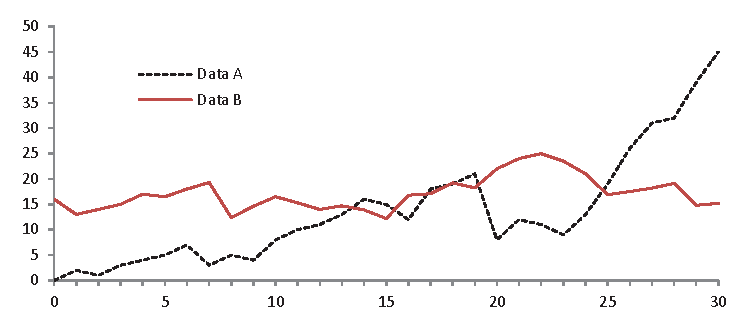
\includegraphics[width=\textwidth]{fig1.eps}
\caption{A figure caption is always placed below the illustration.
Please note that short captions are centered, while long ones are
justified by the macro package automatically.} \label{fig1}
\end{figure}

\begin{theorem}
This is a sample theorem. The run-in heading is set in bold, while
the following text appears in italics. Definitions, lemmas,
propositions, and corollaries are styled the same way.
\end{theorem}
%
% the environments 'definition', 'lemma', 'proposition', 'corollary',
% 'remark', and 'example' are defined in the LLNCS documentclass as well.
%
\begin{proof}
Proofs, examples, and remarks have the initial word in italics,
while the following text appears in normal font.
\end{proof}
For citations of references, we prefer the use of square brackets
and consecutive numbers. Citations using labels or the author/year
convention are also acceptable. The following bibliography provides
a sample reference list with entries for journal
articles~\cite{ref_article1}, an LNCS chapter~\cite{ref_lncs1}, a
book~\cite{ref_book1}, proceedings without editors~\cite{ref_proc1},
and a homepage~\cite{ref_url1}. Multiple citations are grouped
\cite{ref_article1,ref_lncs1,ref_book1},
\cite{ref_article1,ref_book1,ref_proc1,ref_url1}.
\section{SYSTEM MODEL}
\subsection{signal transmission model}
\par
The N-HARQ transmission scheme operates as follows:In the case of successful decoding, an ACK signal is returned to the transmitter, allowing the transmission of subsequent messages.If decoding fails, a NACK signal is returned to the transmitter, triggering a retransmission process.Compared to traditional HARQ, N-HARQ incorporates new information into the original message during retransmissions by leveraging error localization. To mitigate the impact of poor transmission environments, the maximum number of transmissions is set to k. Let $x_k$ denote the new information introduced in the k-th round of the N-HARQ scheme.In the k-th HARQ round, the received signal can be expressed as a superposition of the current information and previously erroneous information in the power domain. Specifically, the received signal at the k-th round is formulated as:
$$
y_k=h_k\sum_{m=1}^k{\sqrt{\alpha _{k,m}p_k}x_k+z_k}\ \ \left( 1 \right) 
$$
\par
$h_k$ represents the channel coefficient between the receiver and the transmitter.$p_k$ denotes the average power of the k-th transmission.$z_k$ stands for the complex additive Gaussian noise with zero mean and variance.$\alpha_{k,m}$ is the power allocation coefficient which satisfies $\sum_{m=1}^k{\alpha _{k,m}}=1$ .The N-HARQ process will terminate only when all messages have been successfully decoded or the maximum HARQ round k is reached.
\par
In real-world scenarios, communication systems inevitably suffer from hardware impairments, channel estimation errors, and feedback delays, making it challenging to obtain perfect channel state information (CSI). Given this context, this paper considers that channel estimation and statistical CSI errors contribute to an imperfect CSI model. Consequently, the actual channel can be modeled as
$$
h_k=\overline{h_k}+\Delta h_k
$$
\par
$\overline{h_k}$ denotes the estimated channel coefficient.$\Delta h_k$ represents the statistical channel estimation error, following a complex Gaussian distribution with zero mean and variance $\sigma _{\varDelta}^{2}$.

\subsection{performance metric}
\par
$Outage\ Probability$: In the N-HARQ protocol, the original information from previously failed transmissions is combined with new messages using a superposition scheme. The received signals are then decoded via a Successive Interference Cancellation (SIC) scheme. Under general assumptions, newer messages are decoded first, with the majority of power allocated to them to ensure lower latency.Let  $C_{i,j}$ denote the event that the accumulated mutual information for the j-th message in the i-th N-HARQ round meets or exceeds a predefined transmission rate $R_j$. This condition can be mathematically expressed as
$$
C_{i,j}=\left\{ \left. \log _2\left( 1+\sum_{k=j}^i{\frac{\left| h_k \right|^2\alpha _{k,j}p_j}{\sigma ^2+\sum_{m=1}^{j-1}{\left| h_k \right|^2\alpha _{k,m}p_k}}}\ge R_j \right) \right\} \right. 
$$
According to the principles of information theory, the outage probability for the i-th HARQ round is denoted as 
\par
$$
P_{out,i}=Pr\left( C_{1,1}^{-}\cap ...\cap \left( C_{i,1}^{-}\cup ...\cup C_{i,i}^{-} \right) \right) 
$$
\par
$C_{i,j}^{-}$ is the complement of $C_{i,j}$. Specifically, it represents the situation where the accumulated important information falls below the required transmission rate. Conventionally,we denote $P_{out,0}=1$
\par
$Long\ Term\ Average\ Throughput$: The Long Term Average Throughput (LTAT) serves as a metric for measuring the transmission efficiency of the N-HARQ protocol. By invoking the renew-reward theory, the long-term average throughput (LTAT) of N-HARQ can be mathematically expressed as
$$
\eta =\frac{\sum_{k=1}^K{R_k\left( P_{out,k-1}-P_{out,K} \right)}}{1+\sum_{k=1}^{K-1}{P_{out,k}}}
$$
\subsection{problem formulation}
To improve transmission efficiency while ensuring energy consumption and transmission reliability, we have formulated the following optimization problem by designing a power allocation strategy for N-HARQ multi-round transmission
$$
\ \ \begin{array}{c}
	\max\\
	p_1,...,p_k\\
\end{array}\eta \ \ \ \ \ \ \ \ s.t.\begin{array}{c}
	C1:p_k\le \bar{p}\\
	C2:p_{avg}\le \bar{p}\\
	C3:P_{out,K}\le \varepsilon\\
\end{array}
$$
\par
$C1$ specifies the maximum transmission power for the k-th round.$C2$  indicates that the average power does not exceed the given limit$\bar{p}$.The average power pavg is calculated as:
\par
$$
p_{avg}=\sum_{k=1}^K{p_kP_{out,k-1}}
$$
\par
$C3$ ensures that the interruption probability of the last round transmission is lower than the predefined $\varepsilon$, which represents the maximum acceptable tolerance for the interruption probability.
\par
The complex mechanism of N-HARQ makes it difficult to derive an explicit expression for the outage probability, which poses high demands on optimization. When traditional optimization techniques fail to provide efficient solutions, employing deep learning to enhance the efficiency of wireless networks is a promising approach. We adopt a novel evaluation network and three attractive power allocation strategies based on deep learning.
\par
To address the challenge of deriving explicit expressions, we use a method that combines the concept of digital twins with a deep neural network-based dual evaluation network. This network takes resource allocation power and channel response as inputs and outputs an approximate outage probability. The core of the network lies in leveraging the universal approximation capability of deep neural networks to estimate the outage probability of N-HARQ. The training data is derived from analyzing the outage probability of N-HARQ transmissions and using information theory principles. The trained dual evaluation network is then used to assess the outage probabilities under different strategies.
\par
We use a supervised learning approach to fit the outage probability under a given power variation configuration. The key to this process lies in selecting and obtaining appropriate data and labels. We use Monte Carlo simulations to generate the outage probabilities of sample data and use these probabilities as labels for training.Specifically,for each data set instance $S^{\left( i \right)}$, a set of transmission power $\left[ p_1,p_2,...,p_K \right] $ and channel coefficient $\left[ \left| h_1 \right|,\left| h_2 \right|,...,\left| h_K \right| \right] $ is given.The corresponding interruption probability $\left[ P_{out,1}^{sim},P_{out,2}^{sim},...,P_{out,K}^{sim} \right]$ can be obtained through Monte Carlo simulation.Use these simulated interruption probabilities as the result labels for $S^{\left( i \right)}$ and denote them as followed.
$$
O^{\left( i \right)}=\left[ P_{out,1}^{sim},P_{out,2}^{sim},...,P_{out,K}^{sim} \right] 
$$
\par
In the dataset $\mathcal{M}$ generated from the i-th training sample, it can be expressed as $O^{\left( i \right)}$ and $S^{\left( i \right)}$.To enhance the network’s predictive accuracy and convergence
rate, we apply a simple transformation to the sample label $O^{\left( i \right)}$
as
\par
$$
\widetilde{O}_k=\log _2\left( -\log _2\left( O_k \right) \right) 
$$
\par
$\widetilde{O}_k$denotes the processed label derived from the original training data label $ O_k $.
\par
The interruption probability $P_{out,k}$ can be predicted by performing specific transformation calculations on the output $\tilde{O}_{k,pre}\$ of the twin evaluation network.
\par
$$
P_{out,k}=2^{-2^{\tilde{O_{k,pre}}}}
$$
\par
The MSE loss function Lop is employed to tune the parameters
of the twin evaluation network, given by
$$
\mathcal{L}_{op}=\frac{1}{\left| \mathcal{M}_{train} \right|*K}\sum_{i=1}^{\left| \mathcal{M}_{train} \right|}{\sum_{k=1}^K{\left( \widetilde{O}_{k}^{\left( i \right)}-\widetilde{O}_{k,pre}^{\left( i \right)} \right) ^2}}
$$
\par
$\left| \mathcal{M}_{*} \right|$ represents the data size of the corresponding data
set.$ \widetilde{O}_{k}^{\left( i \right)}$ and $\widetilde{O}_{k,pre}^{\left( i \right)}$represent the k-th original and predicted labels corresponding to the i-th sample, respectively.
\par
After training, the dual evaluation network can estimate the corresponding outage probability by utilizing real data of power and channel coefficients in a virtual environment, thereby achieving digital twin evaluation.
\section{deep-learning enabled power allocation strategy}
Three deep learning models are adopted to enable power allocation strategies,  
\section{NUMERICAL SIMULATION EXPERIMENTS}

\subsubsection{Acknowledgements} Please place your acknowledgments at
the end of the paper, preceded by an unnumbered run-in heading (i.e.
3rd-level heading).

%
% ---- Bibliography ----
%
% BibTeX users should specify bibliography style 'splncs04'.
% References will then be sorted and formatted in the correct style.
%
% \bibliographystyle{splncs04}
% \bibliography{mybibliography}
%
\begin{thebibliography}{8}
\bibitem{ref_article1}
Author, F.: Article title. Journal \textbf{2}(5), 99--110 (2016)

\bibitem{ref_lncs1}
Author, F., Author, S.: Title of a proceedings paper. In: Editor,
F., Editor, S. (eds.) CONFERENCE 2016, LNCS, vol. 9999, pp. 1--13.
Springer, Heidelberg (2016). \doi{10.10007/1234567890}

\bibitem{ref_book1}
Author, F., Author, S., Author, T.: Book title. 2nd edn. Publisher,
Location (1999)

\bibitem{ref_proc1}
Author, A.-B.: Contribution title. In: 9th International Proceedings
on Proceedings, pp. 1--2. Publisher, Location (2010)

\bibitem{ref_url1}
LNCS Homepage, \url{http://www.springer.com/lncs}. Last accessed 4
Oct 2017
\end{thebibliography}
\end{document}
